\documentclass[10pt]{article}  

\usepackage[catalan]{babel}
\usepackage[utf8]{inputenc}  
\usepackage{graphicx}
\usepackage{color}
\usepackage{float}
\usepackage{caption}

\usepackage{anysize}
\marginsize{2cm}{2cm}{2cm}{2cm} % Izquierda, derecha, arriba, abajo

\usepackage[colorlinks=true,plainpages=true,citecolor=blue,linkcolor=black]{hyperref}

% Para agregar encabezado y pie de página
\usepackage{fancyhdr} 
\pagestyle{fancy}
\fancyhf{}
\fancyhead[L]{\footnotesize XARXES I COMUNICACIONS} %encabezado izquierda
\fancyhead[R]{\footnotesize EPS-UdL}   % dereecha
\fancyfoot[R]{\footnotesize Pràctica 1}  % Pie derecha
\fancyfoot[C]{\thepage}
\fancyfoot[L]{\footnotesize Grau en Enginyeria Informàtica}  %izquierda
\renewcommand{\footrulewidth}{0.4pt}

%%%%%%%% TERMINA PREÁMBULO %%%%%%%%%%%%

\begin{document}
\thispagestyle{empty}

%%%%%%%%%%%%%%%%%%%%%%%%%%%%%%%%%% PORTADA %%%%%%%%%%%%%%%%%%%%%%%%%%%%%%%%%%%%%%%%%%%%
                                                                                    %%%
\begin{center}                                                                      %%%
\newcommand{\HRule}{\rule{\linewidth}{0.5mm}}                                   %%%\left
                                                                                    %%%
\begin{minipage}{0.48\textwidth} \begin{flushleft}

\includegraphics[scale = 0.23]{Images/logo_udl.jpg}
\end{flushleft}\end{minipage}
\begin{minipage}{0.48\textwidth} \begin{flushright}

\includegraphics[scale = 0.25]{Images/logo_eps.jpg}
\end{flushright}\end{minipage}

                                                                                    %%%
\vspace*{-1.5cm}                                %%%
                                                                                    %%% 
\textsc{\huge ESCOLA POLIT\` ECNICA \\ \vspace{5px}SUPERIOR}\\[1.5cm] 

\textsc{\LARGE XARXES I COMUNICACIONS}\\[1.5cm]                                                   %%%

\begin{minipage}{0.9\textwidth} 
\begin{center}                                                                                  %%%
\textsc{\LARGE PR\`ACTICA 1}
\end{center}
\end{minipage}\\[0.5cm]
%%%
                                                                                    %%%
            \vspace*{1cm}                                                                       %%%
                                                                                    %%%
\HRule \\[0.4cm]                                                                    %%%
{ \huge \bfseries RIP, OSPF \& BGP}\\[0.4cm]  %%%
                                                                                    %%%
\HRule \\[1.5cm]                                                                    %%%
                                                                                %%%
                                                                                    %%%
\begin{minipage}{0.46\textwidth}                                                    %%%
\begin{flushleft} \large                                                            %%%
\emph{Students:}\\   
Nil Agut Marín\\
Jaume Giralt Barbé
%%%
            %\vspace*{2cm}  
                                                                %%%
                                                                %%%
\end{flushleft}                                                                     %%%
\end{minipage}      
                                                                %%%
\begin{minipage}{0.52\textwidth}        
\vspace{-0.6cm}                                         %%%
\begin{flushright} \large                                                           %%%
\emph{Professor:} \\                                                                 %%%
Fernández Camon, Cèsar                                                    %%%
\end{flushright}                                                                    %%%
\end{minipage}  
\vspace*{1cm}
%\begin{flushleft}
    

\begin{center}                                                                                  
{\large \today}                                                                 %%%
            \end{center}                                                                        
\end{center}                                                                        
                                                                                    
\newpage                                                                        
%%%%%%%%%%%%%%%%%%%% TERMINA PORTADA %%%%%%%%%%%%%%%%%%%%%%%%%%%%%%%%

\tableofcontents
\listoffigures 
\listoftables

\newpage
\section{Objectius}
L'objectiu principal d'aquesta pràctica és implementar els protocols apresos a classe per a encaminament intern i extern. Per fer l'encaminament intern, utilitzarem els protocols \textbf{RIP} i \textbf{OSPF}. Per a l'encaminament extern farem ús del protocol \textbf{BGP}.
\section{RIP}
És un protocol de porta d'enllaç interna o IGP (Internal Gateway Protocol) utilitzat pels routers (encaminadors), encara que també poden actuar en equips, per intercanviar informació sobre de xarxes IP. En aquest exercici haurem de realitzar unes preguntes sobre el protocol RIP i sobre el seu funcionament. 
\subsection{Topologia de la xarxa}
\begin{figure}[H]
\begin{center}
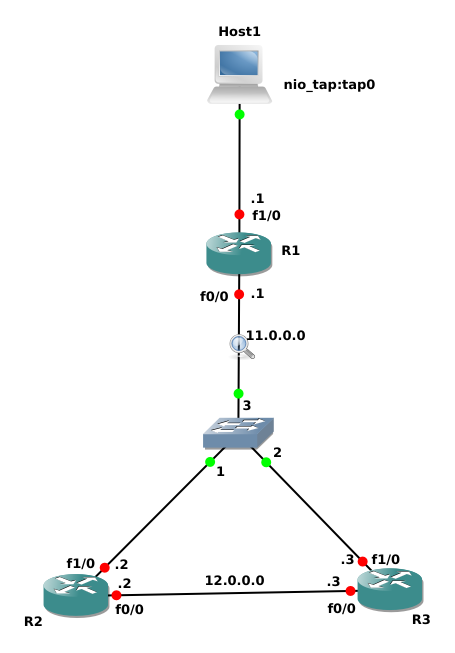
\includegraphics[scale=0.7]{Images/rip.png}
\caption{RIP - Topologia de la xarxa a efectuar l'exercici}
\end{center}
\end{figure}
Per a la realització de aquest exercici utilitzarem encaminadors \textbf{Cisco c7200}
\subsection{Temps de actualització, rutes invàlides i rutes eliminades per defecte}
A continuació, fent ús del programa Wireshark i de comandes al encaminador Cisco, hem de demostrar els diferents temps que té el protocol RIP per actualitzar rutes, marcar-les com invàlides i eliminar-les.
\\\\
En la següent imatge podem veure com els temps d'actualització s'envien cada 30 segons:
\begin{figure}[H]
\begin{center}
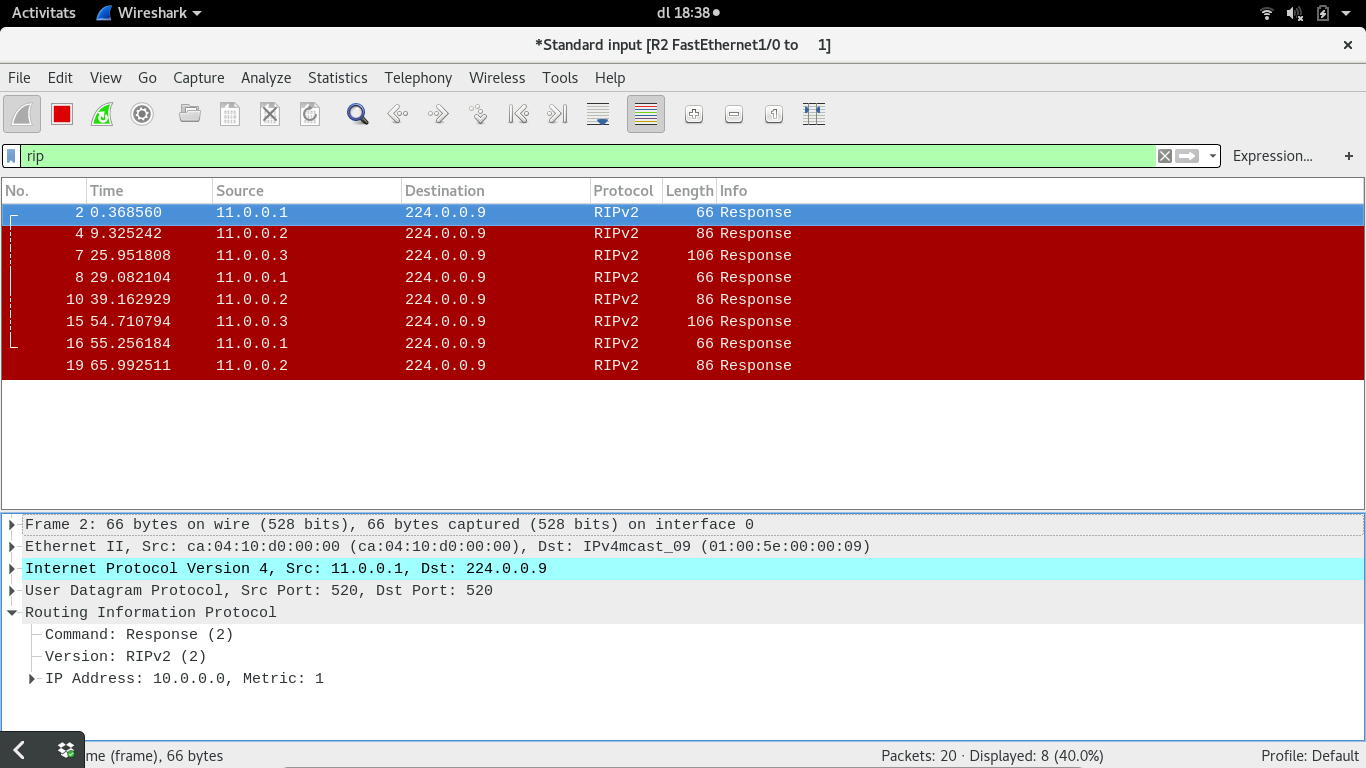
\includegraphics[scale=0.3]{Images/RIP-update.png}
\caption{RIP - Temps d'actualització}
\end{center}
\end{figure}
En la següent imatge s'observa que per defecte, el protocol RIP marca la ruta com invàlida passats 180 segons sense rebre cap paquet d'actualització. En la primera imatge podem veure la hora a la qual hem tancat el encaminador i la seva taula d'encaminament RIP i en la segona imatge podem veure que han passat uns 180 segons i en la seva taula podem veure que hi ha marcat que la ruta és possible que sigui invàlida.
\begin{figure}[H]
\begin{center}
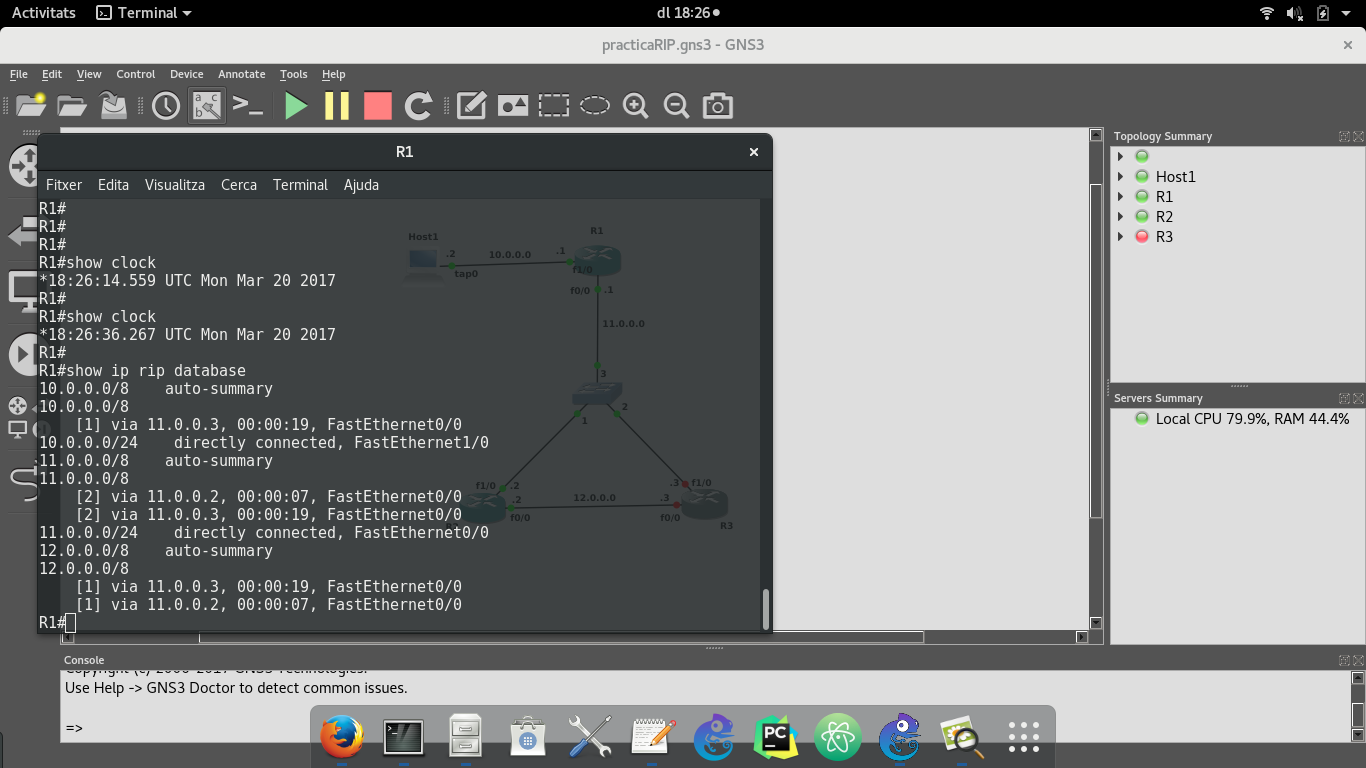
\includegraphics[scale=0.3]{Images/RIP-invalid1.png}
\caption{RIP - Temps ruta invàlida}
\end{center}
\end{figure}
\begin{figure}[H]
\begin{center}
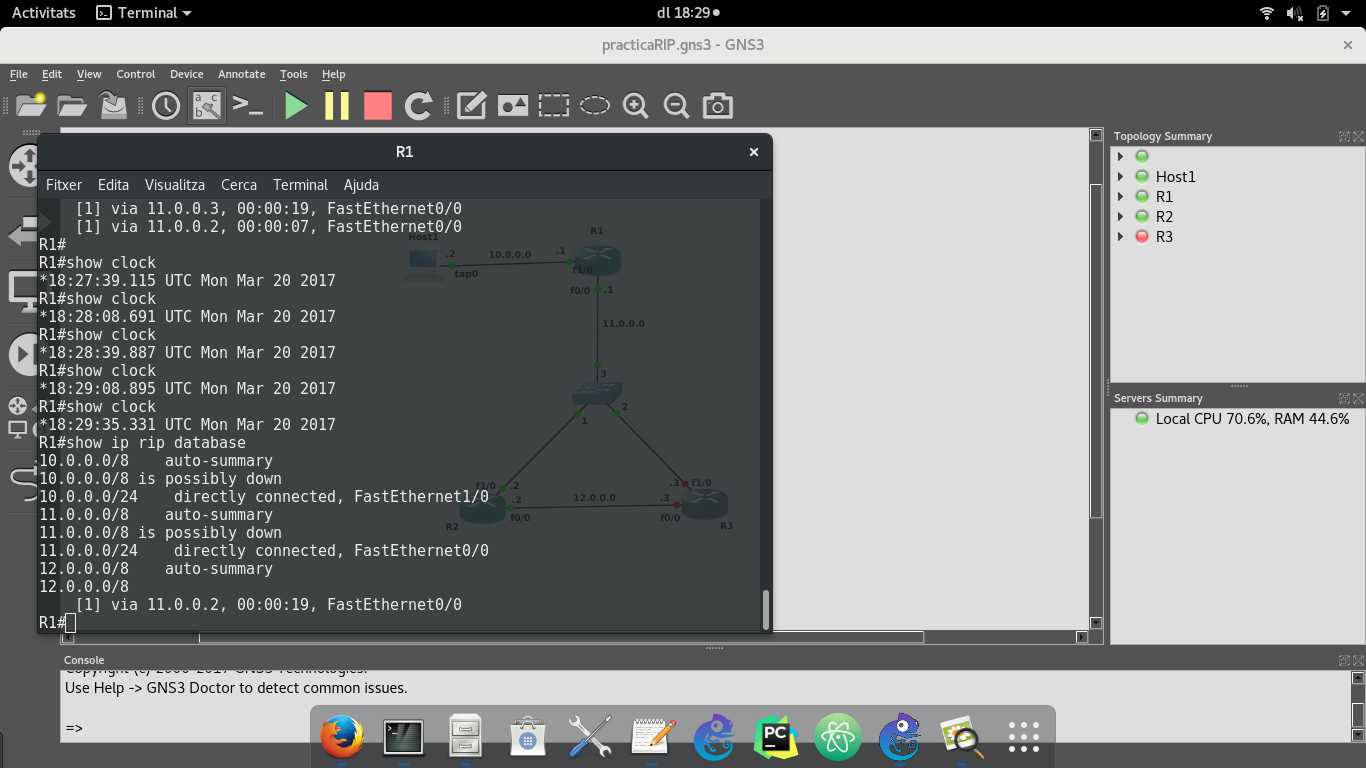
\includegraphics[scale=0.3]{Images/RIP-invalid2.png}
\caption{RIP - Temps ruta invàlida}
\end{center}
\end{figure}
Finalment, en la següent imatge podem veure com després de 240 segons sense cap paquet d'actualització, el protocol RIP per defecte elimina la ruta de la taula d'encaminament del encaminador.
\begin{figure}[H]
\begin{center}
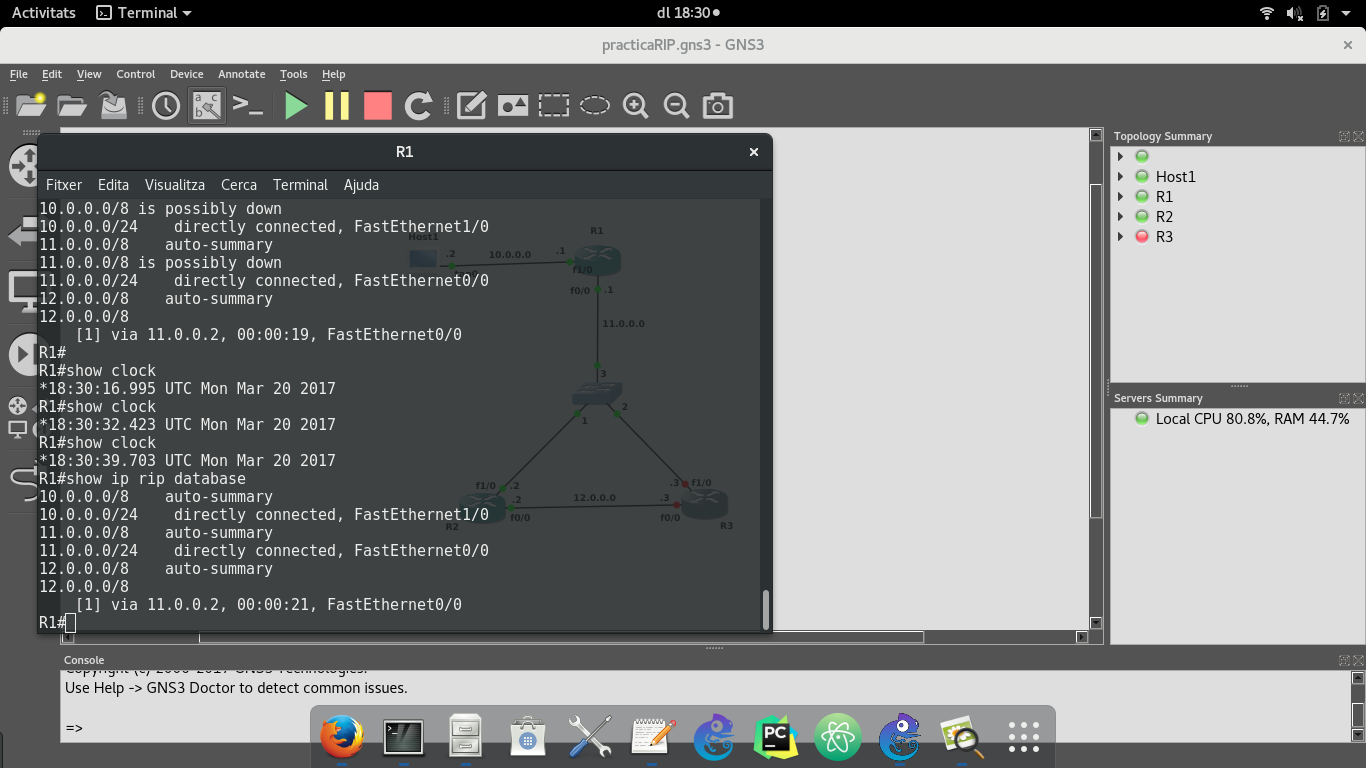
\includegraphics[scale=0.3]{Images/RIP-flush.png}
\caption{RIP - Temps ruta eliminada}
\end{center}
\end{figure}
\subsection{Demostreu que per defecte split-horizon està activat i poison-reverse desactivat}

\subsection{Demostreu el problema  	\textit{count-to-infinity} en la xarxa}
Després de desactivar split-horizon per cada interfície de la xarxa i canviar els temps per defecte de BGP (actualitzacions cada 2 segons, invalid als 10 segons, hold-time als 0 segons i eliminar la ruta als 20 segons), hem pogut experimentar que si desconnectem el encaminador R1 és pot produir el problema \textit{count-to-infinity}.
\section{OSPF}
És un protocol d'encaminament d'estat d'enllaç considerat de porta d'enllaç interna. Utilitza codi obert i envia els paquets primer pel camí més curt. Fa ús de l'algoritme SPF que es basa principalment en el valor de l'amplada de banda de les connexions.
\subsection{Topologia de la xarxa}
\begin{figure}[H]
\begin{center}
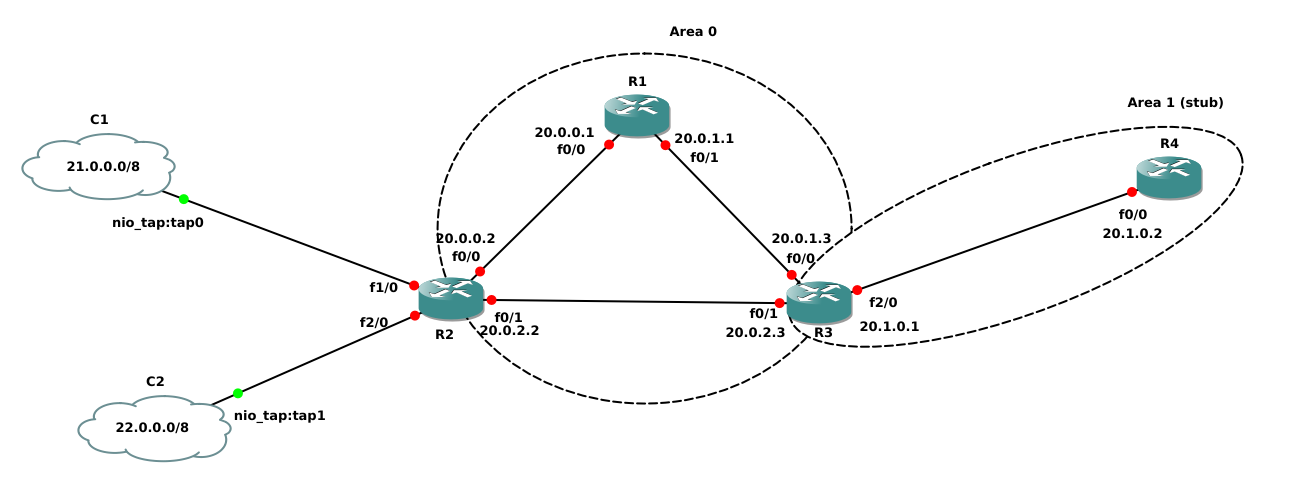
\includegraphics[scale=0.5]{Images/ospf.png}
\caption{Topologia de la xarxa a efectuar l'exercici}
\end{center}
\end{figure}
Per a la realització de aquest exercici utilitzarem encaminadors \textbf{Cisco c7200}. També hem de utilitzar les següents xarxes:
\begin{table}[h!]
\centering
\label{my-label}
\begin{tabular}{|l|l|}
\hline
Instead of: & Use:          \\ \hline
10.0.0.0/24 & X.0.0.0/24    \\ \hline
10.0.1.0/24 & X.0.1.0/24    \\ \hline
10.0.2.0/24 & X.0.2.0/24    \\ \hline
10.1.0.0/24 & X.1.0.0/24    \\ \hline
11.0.0.0/8  & (X+1).0.0.0/8 \\ \hline
12.0.0.0/8  & (X+2).0.0.0/8 \\ \hline
\end{tabular}
\caption{Xarxes a utilitzar en l'exercici OSPF}
\end{table}
\subsection{Imatges de la base de dades OSPF de cada encaminador}
\subsubsection{Encaminador R1}
\begin{figure}[H]
\begin{center}
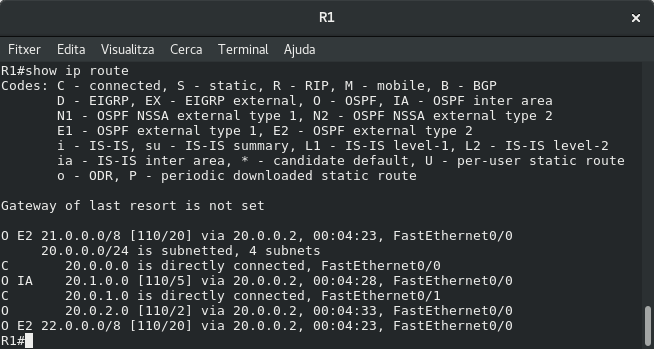
\includegraphics[scale=0.5]{Images/ospf-R1-route.png}
\caption{OSPF - Comanda \textit{show ip route} en el encaminador R1}
\end{center}
\end{figure}
\begin{figure}[H]
\begin{center}
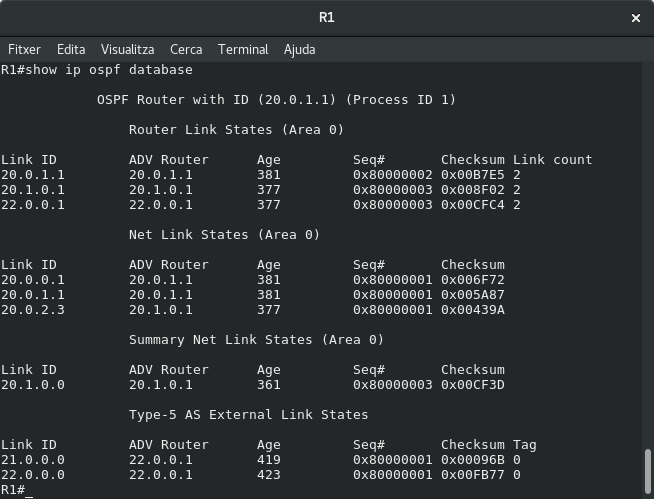
\includegraphics[scale=0.5]{Images/ospf-R1-database.png}
\caption{OSPF - Comanda \textit{show ip ospf database} en el encaminador R1}
\end{center}
\end{figure}
\begin{figure}[H]
\begin{center}
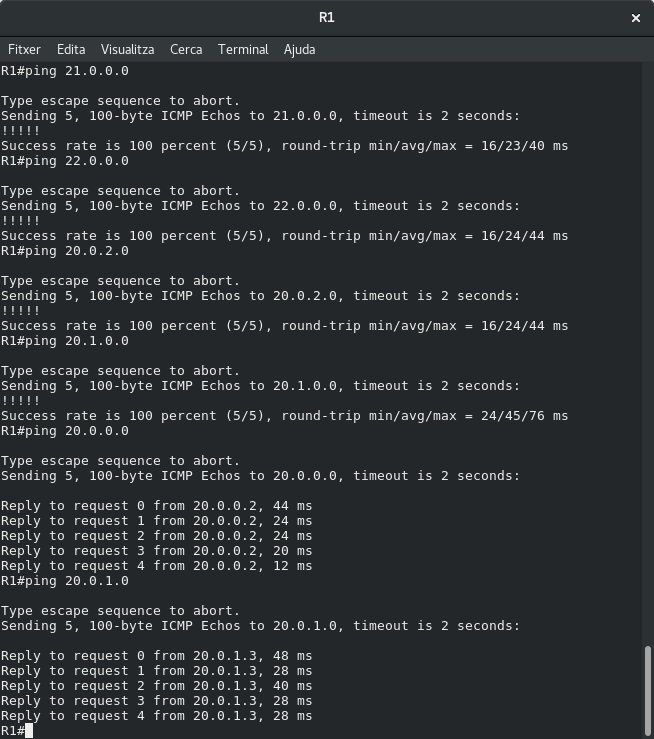
\includegraphics[scale=0.4]{Images/ospf-R1-conectivity.png}
\caption{OSPF - Prova de connectivitat a la xarxa des de l'encaminador R1}
\end{center}
\end{figure}
\subsubsection{Encaminador R2}
\begin{figure}[H]
\begin{center}
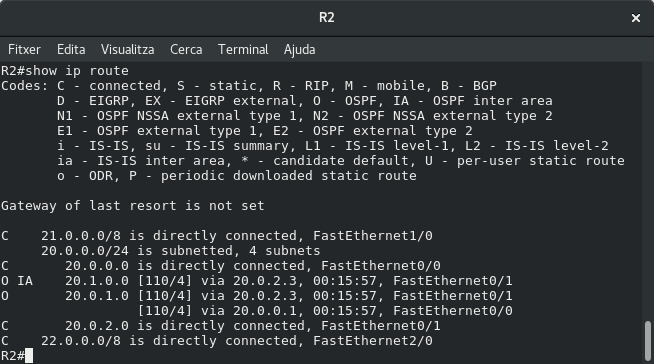
\includegraphics[scale=0.5]{Images/ospf-R2-route.png}
\caption{OSPF - Comanda \textit{show ip route} en el encaminador R2}
\end{center}
\end{figure}
\begin{figure}[H]
\begin{center}
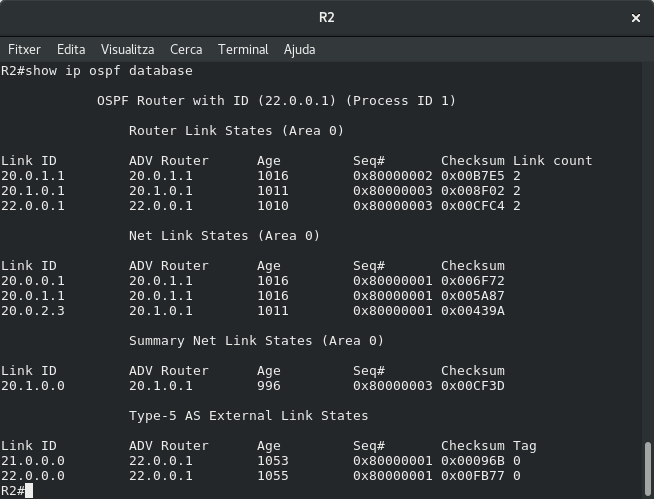
\includegraphics[scale=0.5]{Images/ospf-R2-database.png}
\caption{OSPF - Comanda \textit{show ip ospf database} en el encaminador R2}
\end{center}
\end{figure}
\begin{figure}[H]
\begin{center}
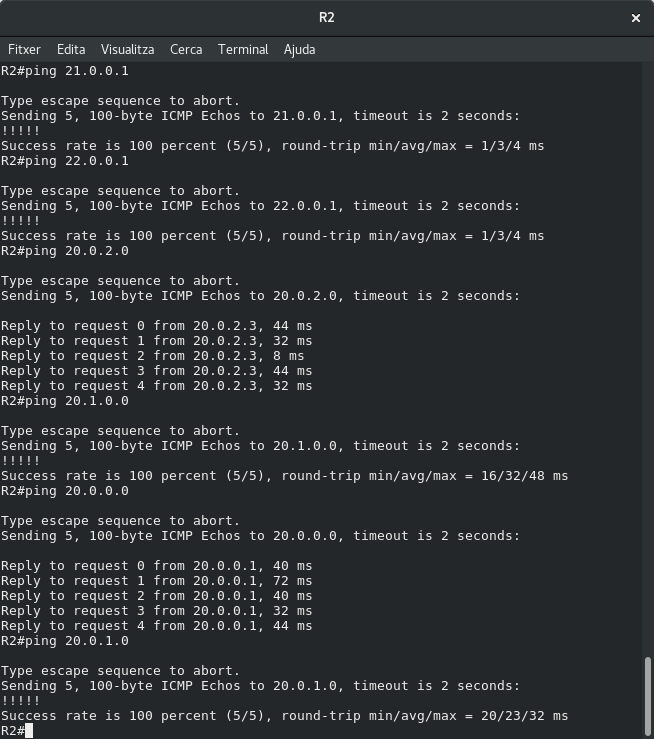
\includegraphics[scale=0.4]{Images/ospf-R2-conectivity.png}
\caption{OSPF - Prova de connectivitat a la xarxa des de l'encaminador R2}
\end{center}
\end{figure}
\subsubsection{Encaminador R3}
\begin{figure}[H]
\begin{center}
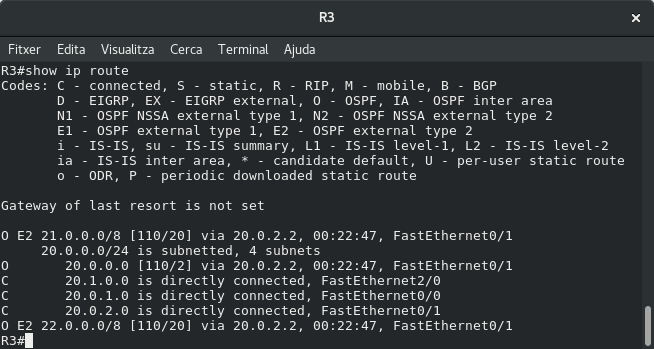
\includegraphics[scale=0.5]{Images/ospf-R3-route.png}
\caption{OSPF - Comanda \textit{show ip route} en el encaminador R3}
\end{center}
\end{figure}
\begin{figure}[H]
\begin{center}
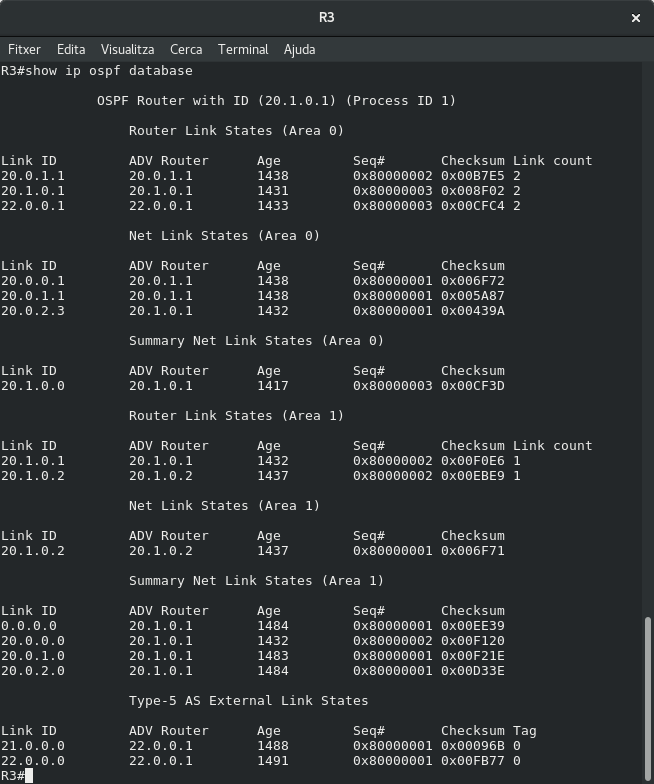
\includegraphics[scale=0.4]{Images/ospf-R3-database.png}
\caption{OSPF - Comanda \textit{show ip ospf database} en el encaminador R3}
\end{center}
\end{figure}
\begin{figure}[H]
\begin{center}
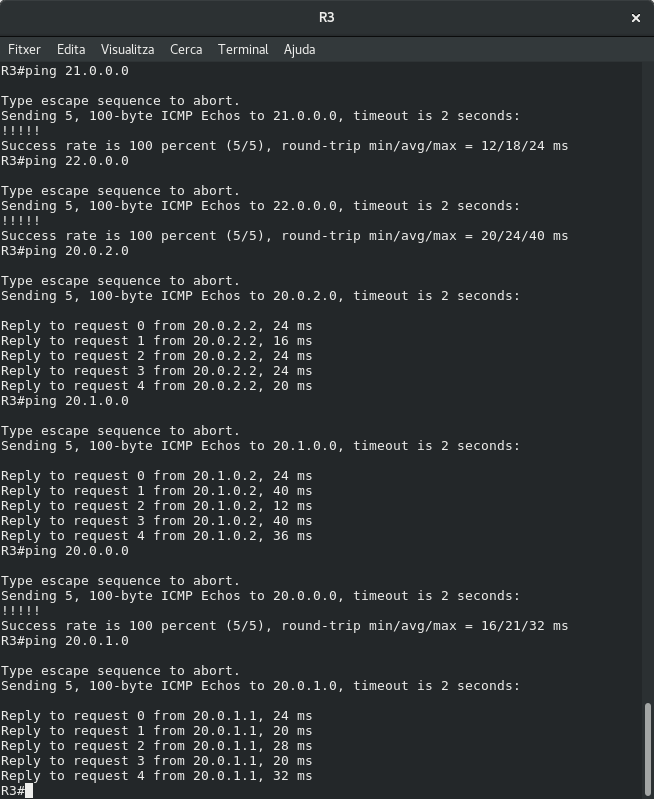
\includegraphics[scale=0.4]{Images/ospf-R3-conectivity.png}
\caption{OSPF - Prova de connectivitat a la xarxa des de l'encaminador R3}
\end{center}
\end{figure}
\subsubsection{Encaminador R4}
\begin{figure}[H]
\begin{center}
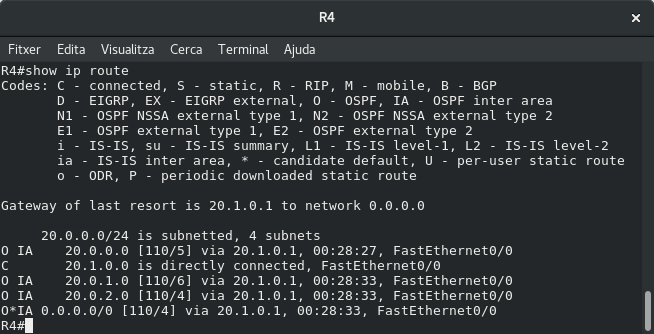
\includegraphics[scale=0.5]{Images/ospf-R4-route.png}
\caption{OSPF - Comanda \textit{show ip route} en el encaminador R4}
\end{center}
\end{figure}
\begin{figure}[H]
\begin{center}
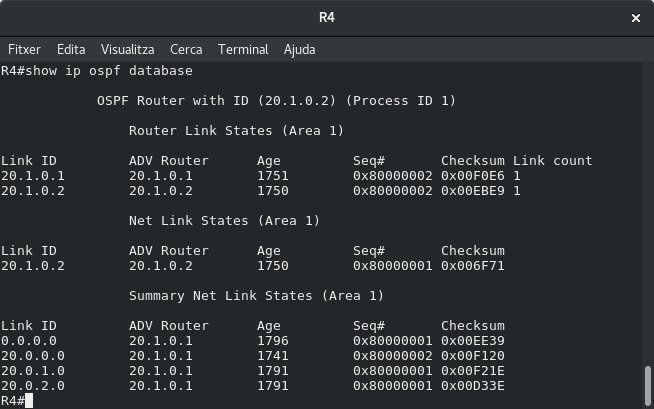
\includegraphics[scale=0.5]{Images/ospf-R4-database.png}
\caption{OSPF - Comanda \textit{show ip ospf database} en el encaminador R4}
\end{center}
\end{figure}
\begin{figure}[H]
\begin{center}
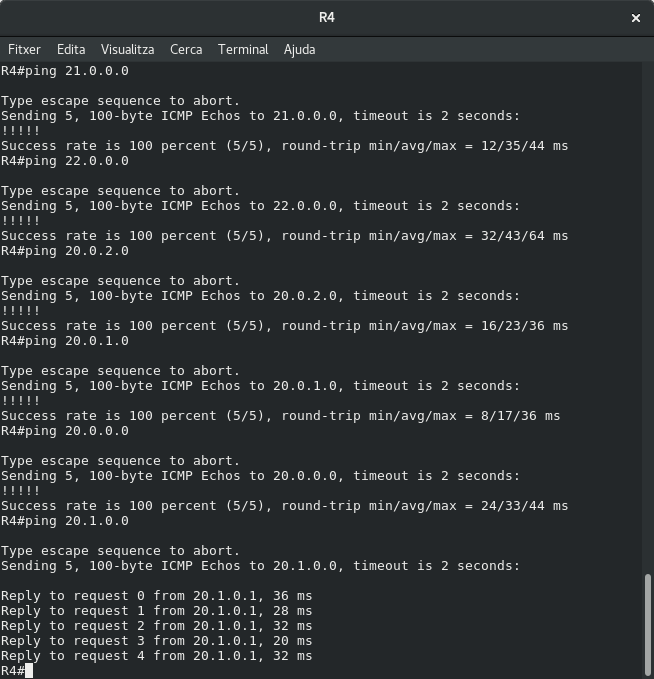
\includegraphics[scale=0.5]{Images/ospf-R4-conectivity.png}
\caption{OSPF - Prova de connectivitat a la xarxa des de l'encaminador R4}
\end{center}
\end{figure}
\section{BGP}
És un protocol de comunicació mitjançant el qual s'intercanvia informació d'encaminament entre sistemes autònoms. Per exemple, els ISP registrats a Internet solen compondre's de diversos sistemes autònoms i per a aquest cas és necessari un protocol com BGP. Entre els sistemes autònoms dels ISP s'intercanvien les seues taules de rutes a través del protocol BGP. Aquest intercanvi d'informació d'encaminament es fa entre els encaminadors externs de cada sistema autònom. Aquests encaminadors han de suportar BGP. Es tracta del protocol més utilitzat per a xarxes amb intenció de configurar un EGP (external gateway protocol)
\subsection{Topologia de la xarxa}
\begin{figure}[H]
\begin{center}
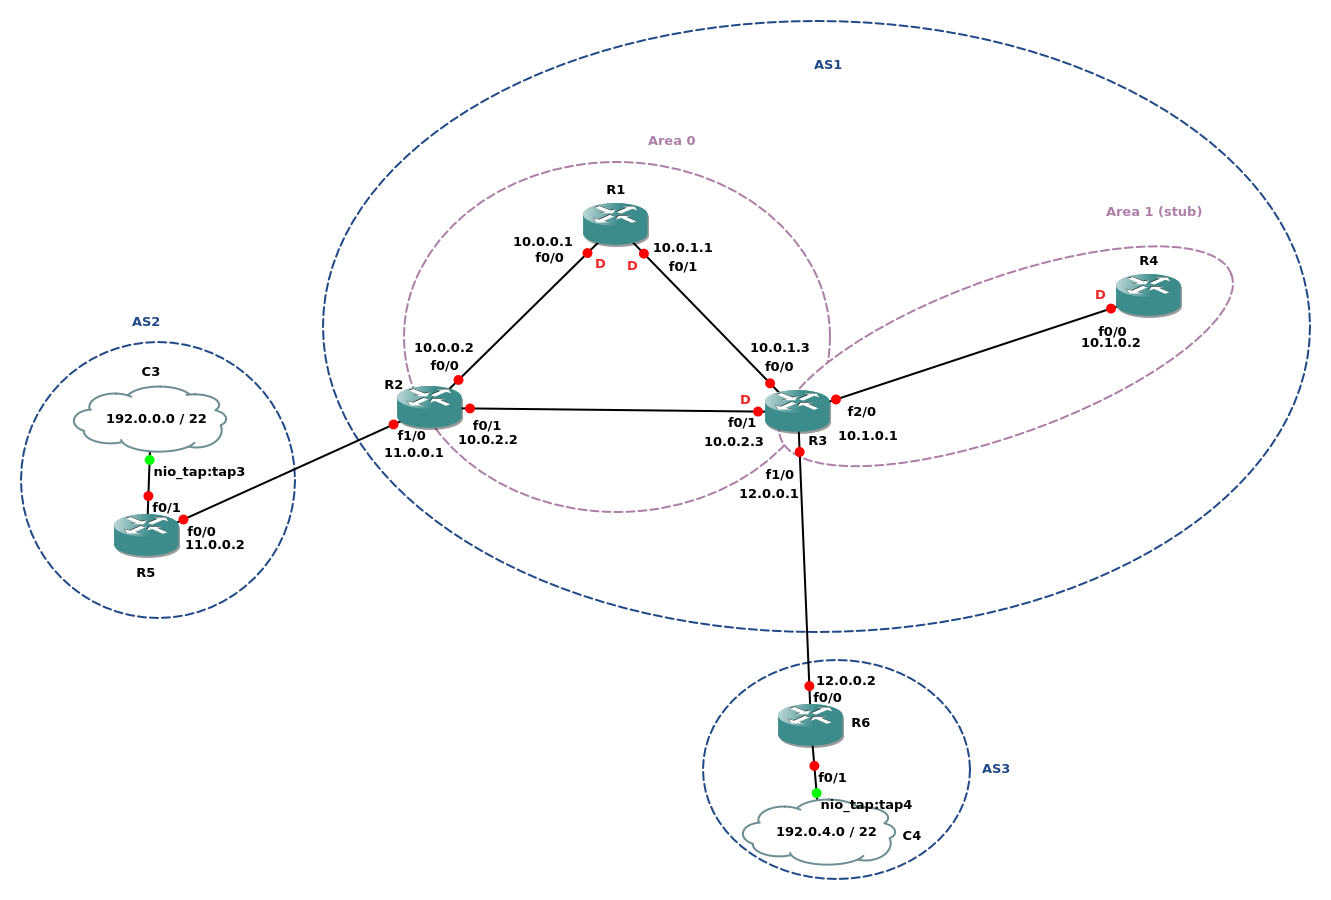
\includegraphics[scale=0.5]{Images/bgp.png}
\caption{BGP - Topologia de la xarxa a efectuar l'exercici}
\end{center}
\end{figure}
Per a la realització de aquest exercici utilitzarem encaminadors \textbf{Cisco c7200}.
\subsection{Connectivitat entre sistemes autònoms}
\subsubsection{Encaminador R6}
\begin{figure}[H]
\begin{center}
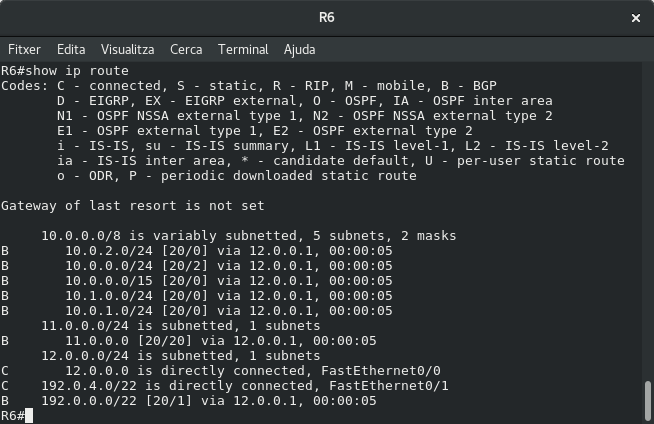
\includegraphics[scale=0.5]{Images/bgp-R6-route.png}
\caption{BGP - Comanda \textit{show ip route} en el encaminador R6}
\end{center}
\end{figure}
\begin{figure}[H]
\begin{center}
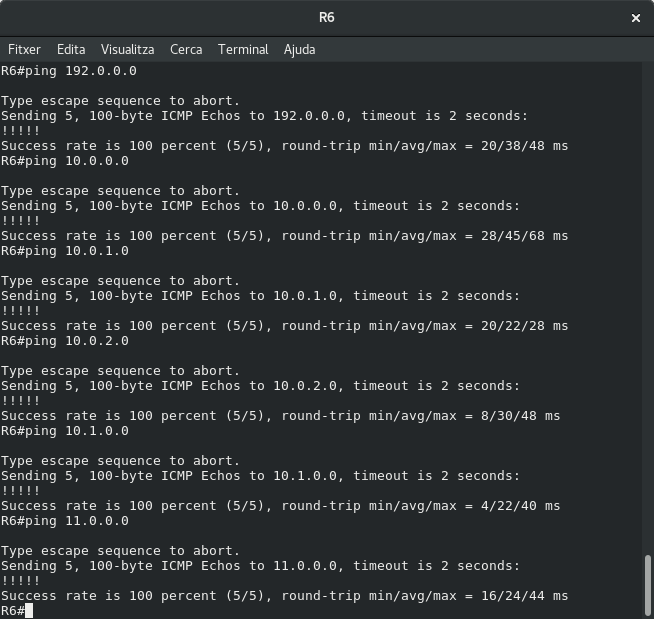
\includegraphics[scale=0.5]{Images/bgp-R6-conectivity.png}
\caption{BGP - Prova de connectivitat a la xarxa des de l'encaminador R6}
\end{center}
\end{figure}
\subsubsection{Encaminador R5}
\begin{figure}[H]
\begin{center}
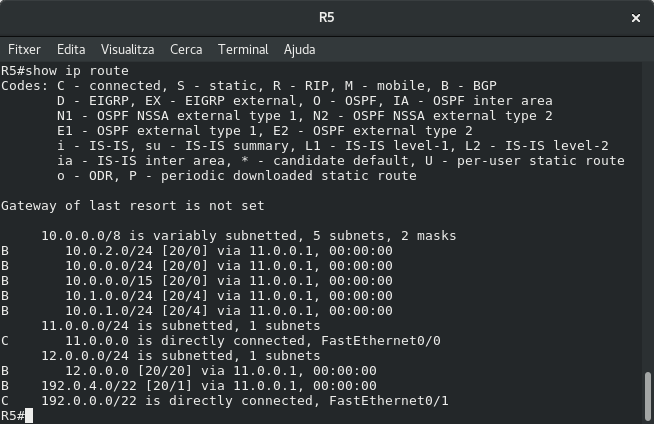
\includegraphics[scale=0.5]{Images/bgp-R5-route.png}
\caption{BGP - Comanda \textit{show ip route} en el encaminador R5}
\end{center}
\end{figure}
\begin{figure}[H]
\begin{center}
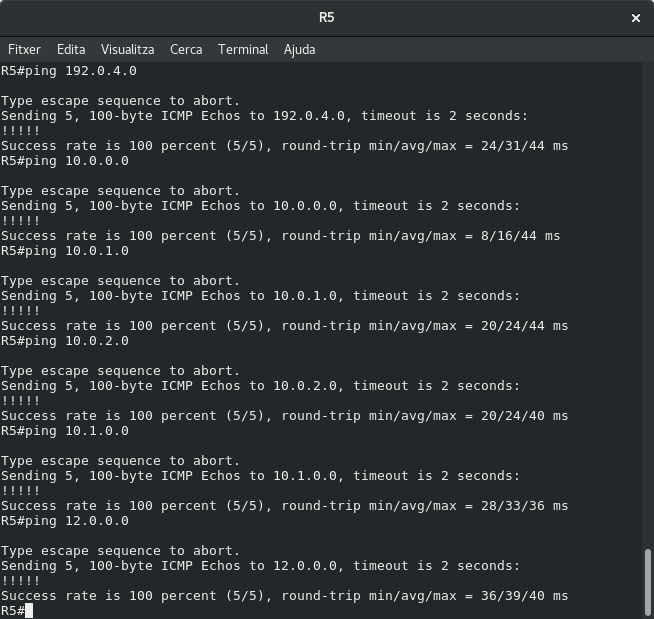
\includegraphics[scale=0.5]{Images/bgp-R5-conectivity.png}
\caption{BGP - Prova de connectivitat a la xarxa des de l'encaminador R5}
\end{center}
\end{figure}
\subsubsection{Encaminador R1}
\begin{figure}[H]
\begin{center}
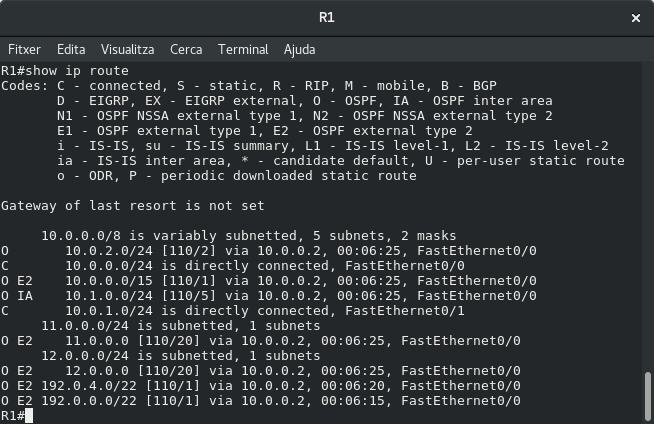
\includegraphics[scale=0.4]{Images/bgp-R1-route.png}
\caption{BGP - Comanda \textit{show ip route} en el encaminador R1}
\end{center}
\end{figure}
\begin{figure}[H]
\begin{center}
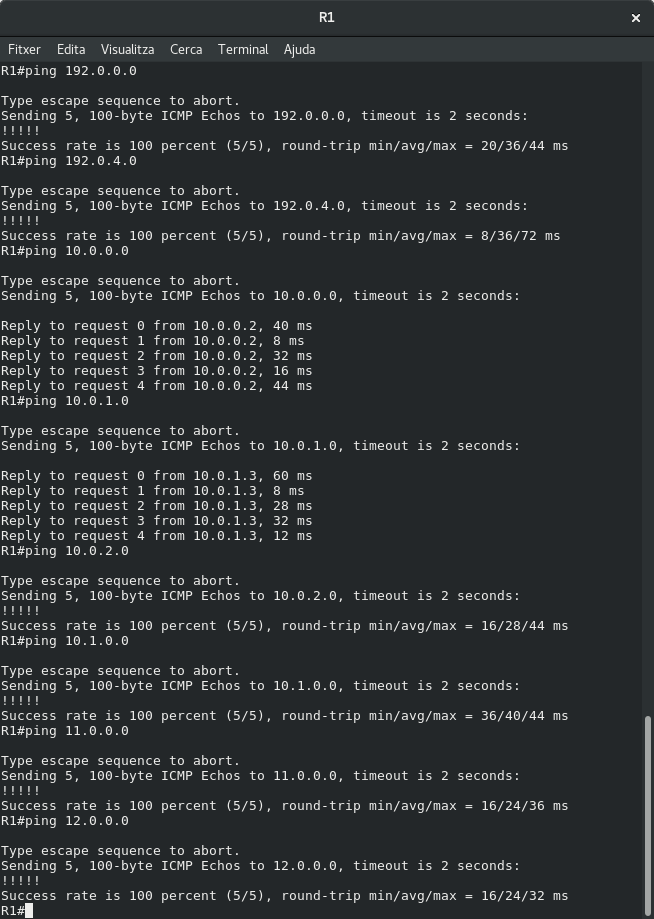
\includegraphics[scale=0.4]{Images/bgp-R1-conectivity.png}
\caption{BGP - Prova de connectivitat a la xarxa des de l'encaminador R1}
\end{center}
\end{figure}
\subsection{Principals problemes a la hora de configurar}
\end{document}
              
